\documentclass[12pt]{book}

\usepackage{mathptm,times,color}
\usepackage[pdftex]{graphicx}
\usepackage{multirow}
\usepackage{bezier}
\usepackage{rotating}
\usepackage{longtable}
\usepackage{amsmath}
\usepackage{xfrac}
\usepackage{array}
\usepackage{units}
\usepackage{fix-cm}
\usepackage{makeidx} % Create index at end of document
\usepackage[nottoc,notlof,notlot]{tocbibind} % Put the bibliography and index in the ToC
\usepackage{datetime}
\newdateformat{mydate}{\monthname[\THEMONTH] \THEYEAR}

\usepackage{listings}
\usepackage{textcomp}
\definecolor{lbcolor}{rgb}{0.96,0.96,0.96}
\lstset{
    %backgroundcolor=\color{lbcolor},
    tabsize=4,
    rulecolor=,
    language=Fortran,
        basicstyle=\footnotesize\ttfamily,
        upquote=true,
        aboveskip={\baselineskip},
        belowskip={\baselineskip},
        columns=fixed,
        extendedchars=true,
        breaklines=true,
        breakatwhitespace=true,
        frame=none,
        showtabs=false,
        showspaces=false,
        showstringspaces=false,
        identifierstyle=\ttfamily,
        keywordstyle=\color[rgb]{0,0,0},
        commentstyle=\color[rgb]{0,0,0},
        stringstyle=\color[rgb]{0,0,0},
}

\usepackage{wrapfig}
\usepackage{morefloats}

\newcolumntype{L}[1]{>{\raggedright\let\newline\\\arraybackslash\hspace{0pt}}m{#1}}
\newcolumntype{C}[1]{>{\centering\let\newline\\\arraybackslash\hspace{0pt}}m{#1}}
\newcolumntype{R}[1]{>{\raggedleft\let\newline\\\arraybackslash\hspace{0pt}}m{#1}}

\usepackage{framed}
\newcommand{\graybox}[1]{
\begin{shaded}#1\end{shaded}
}

\renewcommand{\bibname}{References}

% dummy change to force revision update

%\usepackage{eso-pic}
%\usepackage{graphicx}
%\usepackage{color}
%\usepackage{type1cm}


%\makeatletter
%   \AddToShipoutPicture{%
%     \setlength{\@tempdimb}{.5\paperwidth}%
%    \setlength{\@tempdimc}{.5\paperheight}%
%   \setlength{\unitlength}{1pt}%
%  \put(\strip@pt\@tempdimb,\strip@pt\@tempdimc){%
%     \makebox(0,0){\rotatebox{45}{\textcolor[gray]{0.75}{\fontsize{8cm}{8cm}\selectfont{DRAFT}}}}}}
%\makeatother

\definecolor{linknavy}{rgb}{0,0,0.50196}
\definecolor{linkred}{rgb}{1,0,0}
\definecolor{linkblue}{rgb}{0,0,1}
\definecolor{shadecolor}{rgb}{0.9,0.9,0.9}

\usepackage[pdftex,
        colorlinks=true,
        urlcolor=linkblue,     % \href{...}{...} external (URL)
        citecolor=linkred,     % citation number colors
        linkcolor=linknavy,    % \ref{...} and \pageref{...}
        pdfproducer={pdflatex},
        pagebackref,
        pdfpagemode=UseNone,
        bookmarksopen=true,
        plainpages=false,
        verbose]{hyperref}

% CFAST Version String
\newcommand{\cfastversion}{7.0.0}

% commands to use for "official" cover and title pages
% see smokeview verification guide to see how they are used

\newcommand{\logosigs}{
\begin{minipage}[b]{6.5in}
\flushright{
\includegraphics[height=1.05in]{FIGURES/nistident}}
\end{minipage}
}

\newcommand{\titlesigs}
{
\small
\begin{flushright}
U.S. Department of Commerce \\
{\em Penny Pritzker, Secretary} \\
\hspace{1in} \\
National Institute of Standards and Technology \\
{\em Willie May, Acting Under Secretary of Commerce for Standards and Technology and Acting Director}
\end{flushright}
}

\newcommand{\headerA}[1]{
\begin{flushright}
\fontsize{20}{24}\selectfont
\bf{NIST Technical Note #1}
\end{flushright}
}


\newcommand{\headerB}[1]{
\begin{flushright}
\fontsize{28}{33.6}\selectfont
\bf{#1}
\end{flushright}
}

\newcommand{\headerC}[1]{
\vspace{.15in}
\begin{flushright}
\fontsize{12}{14}\selectfont
#1
\end{flushright}
}

\newcommand{\headerD}[1]{
\begin{flushright}
\fontsize{12}{14}\selectfont
This publication is available free of charge from: \\
http://dx.doi.org/10.6028/NIST.TN.#1
\end{flushright}
}



\setlength{\textwidth}{6.5in}
\setlength{\textheight}{9.0in}
\setlength{\topmargin}{0.in}
\setlength{\headheight}{0.in}
\setlength{\headsep}{0.in}
\setlength{\parindent}{0.25in}
\setlength{\oddsidemargin}{0.0in}
\setlength{\evensidemargin}{0.0in}


\newcommand{\rd}{\mathrm{d}}
\newcommand{\brackets}[1]{ { \left( {#1} \right) } }
\newcommand{\dbydt}[1]{\frac{\rd {#1}}{\rd t}}
\newcommand{\superscript}[1]{\ensuremath{^{\textnormal{\scriptsize \hbox{#1}}}}}
\newcommand{\subscript}[1]{\ensuremath{_{\textnormal{\scriptsize \hbox{#1}}}}}

\newcommand{\textct}[1]{\texttt{\small #1}}

\newcommand{\trho}{\tilde{\rho}}
\newcommand{\chia}{\chi_{\rm a}}
\newcommand{\chir}{\chi_{\rm r}}
\newcommand{\dph}{{\delta\phi}}
\newcommand{\dth}{{\delta\theta}}
\newcommand{\tp}{\tilde{p}}
\newcommand{\dQ}{\dot{Q}}
\newcommand{\dQc}{\dot{Q}_{\rm c}}
\newcommand{\dQr}{\dot{Q}_{\rm r}}
\newcommand{\Dh}{\Delta H}
\newcommand{\DhO}{\Delta H_\OTWO}
\newcommand{\Tp}{T_{\rm p}}
\newcommand{\Tu}{T_{\rm u}}
\newcommand{\Tl}{T_{\rm l}}
\newcommand{\Ts}{T_{\rm s}}
\newcommand{\Tg}{T_{\rm g}}
\newcommand{\TL}{T_{\rm L}}
\newcommand{\Vu}{V_{\rm u}}
\newcommand{\Vl}{V_{\rm l}}
\newcommand{\doh}{\dot{h}}
\newcommand{\dhl}{\dot{h}_{\rm l}}
\newcommand{\dhu}{\dot{h}_{\rm u}}
\newcommand{\dmal}{\dot{m}_{\rm l}}
\newcommand{\dmau}{\dot{m}_{\rm u}}
\newcommand{\dq}{\dot{q}}
\newcommand{\dqc}{\dot{q}_{\rm c}}
\newcommand{\dqr}{\dot{q}_{\rm r}}
\newcommand{\dm}{\dot{m}}
\newcommand{\dme}{\dot{m}_{\rm e}}
\newcommand{\dmp}{\dot{m}_{\rm p}}
\newcommand{\dml}{\dot{m}_{\rm l}}
\newcommand{\dmu}{\dot{m}_{\rm u}}
\newcommand{\dmf}{\dot{m}_{\rm f}}

\newcommand{\be}{\begin{equation}}
\newcommand{\ee}{\end{equation}}

\newcommand{\RE}{\hbox{Re}}
\newcommand{\LE}{\hbox{Le}}
\newcommand{\PR}{\hbox{Pr}}
\newcommand{\PE}{\hbox{Pe}}
\newcommand{\NU}{\hbox{Nu}}
\newcommand{\SC}{\hbox{Sc}}
\newcommand{\SH}{\hbox{Sh}}
\newcommand{\WE}{\hbox{We}}

\newcommand{\COTWO}{{\tiny \hbox{CO}_2}}
\newcommand{\OTWO}{{\tiny \hbox{O}_2}}
\newcommand{\CO}{{\tiny \hbox{CO}}}
\newcommand{\HTWOO}{{\tiny \hbox{H}_2\hbox{O}}}
\newcommand{\NTWO}{{\tiny \hbox{N}_2}}
\newcommand{\F}{{\tiny \hbox{F}}}
\newcommand{\So}{{\tiny \hbox{S}}}
\newcommand{\M}{{\tiny \hbox{M}}}
\newcommand{\HCN}{{\tiny \hbox{HCN}}}
\newcommand{\HCl}{{\tiny \hbox{HCl}}}
\newcommand{\Hy}{{\tiny \hbox{H}}}
\newcommand{\C}{{\tiny \hbox{C}}}
\newcommand{\N}{{\tiny \hbox{N}}}
\newcommand{\Oh}{{\tiny \hbox{O}}}
\newcommand{\Cl}{{\tiny \hbox{Cl}}}

\newcommand{\asqh}{$A_T/A\sqrt{h}$}
\newcommand{\degc}{$^{\circ}$C}
\newcommand{\degf}{$^{\circ}$F}

\newcommand{\dx}{\delta x}
\newcommand{\dy}{\delta y}
\newcommand{\dz}{\delta z}
\newcommand{\dt}{\delta t}

\newcommand{\ha}{\frac{1}{2}}
\newcommand{\ft}{\frac{4}{3}}
\newcommand{\ot}{\frac{1}{3}}
\newcommand{\fofi}{\frac{4}{5}}
\newcommand{\of}{\frac{1}{4}}
\newcommand{\twth}{\frac{2}{3}}

\newcommand{\ct}{\tt\small}

\newcommand{\rb}[1]{\raisebox{1.5ex}[0pt]{#1}}

\newcommand{\erf}{\hbox{erf}}



\begin{document}

\bibliographystyle{unsrt}

\frontmatter

\pagestyle{empty}


\begin{minipage}[t][9in][s]{6.5in}

\headerA{XXXX\\}

\headerB{
CFAST -- Consolidated Fire \\
 and Smoke Transport \\
 (Version 7) \\
 Volume 1: Technical Reference Guide \\
}

\headerC{
   Richard D. Peacock \\
   Kevin B. McGrattan \\
   Glenn P. Forney \\
   Paul A. Reneke \\
}

\vfill

\headerD{XXXXv1}

\vfill

\logosigs

\end{minipage}

\newpage

\hspace{5in}

\newpage

\begin{minipage}[t][9in][s]{6.5in}

\headerA{XXXX\\}

\headerB{
CFAST -- Consolidated Fire \\
 And Smoke Transport \\
 (Version 7) \\
 Volume 1: Technical Reference Guide \\
}

\headerC{
   Richard D. Peacock \\
   Kevin B. McGrattan \\
   Glenn P. Forney \\
   Paul A. Reneke \\
}

\headerD{XXXXv2}

\headerC{
\flushright{\mydate\today\\
CFAST Version \cfastversion \\
\emph{SVN Repository}~$Revision$}}
% dummy comment to force svn change - Mon Jan  5 21:57:14 EST 2015

\vfill

\flushright{
\includegraphics[width=1.2in]{FIGURES/doc} }

\titlesigs

\end{minipage}


\newpage

\frontmatter

\pagestyle{plain}
\setcounter{page}{3}


\chapter{Preface}

This document provides the theoretical basis for the Consolidated Fire And Smoke Transport (CFAST) model, following the general framework set forth in the ``Standard Guide for Evaluating the Predictive Capability of Deterministic Fire Models,'' ASTM~E~1355~\cite{ASTM:E1355}. Instructions for using CFAST are contained in a separate user's guide, and model assessment information is contained in a separate verification and validation guide.

\chapter{Disclaimer}

The US Department of Commerce makes no warranty, expressed or implied, to users of CFAST, and accepts no responsibility for its use. Users of CFAST assume sole responsibility under Federal law for determining the appropriateness of its use in any particular application; for any conclusions drawn from the results of its use; and for any actions taken or not taken as a result of analysis performed using these tools.

Users are warned that CFAST is intended for use only by those competent in the fields of fluid dynamics, thermodynamics, heat transfer, combustion, and fire science, and is intended only to supplement the informed judgment of the qualified user. The software package is a computer model that may or may not have predictive capability when applied to a specific set of factual circumstances. Lack of accurate predictions by the model could lead to erroneous conclusions with regard to fire safety. All results should be evaluated by an informed user.

Throughout this document, the mention of computer hardware or commercial software does not constitute endorsement by NIST, nor does it indicate that the products are necessarily those best suited for the intended purpose.




\chapter{Acknowledgments}

\label{acksection}

CFAST was originally developed by Walter Jones, formerly of NIST.

Continuing support for CFAST is via internal funding at NIST. In addition, support is provided by other agencies of the U.S. Federal Government, most notably the Nuclear Regulatory Commission (NRC) and the Department of Energy (DOE). The NRC Office of Research has funded key validation experiments, the preparation of the CFAST manuals, and the continuing development of sub-models that are of importance in the area of nuclear power plant safety. Special thanks to Mark Salley and David Stroup for their support. Support to refine the software development and quality assurance process for CFAST has been provided by the DOE. The assistance of Subir Sen and Debra Sparkman is gratefully acknowledged.

Doug Carpenter, Combustion Sciences and Engineering, has contributed numerous corrections, clarifications, and updates to the guides and the model through his detailed review of the model and documentation. Allan Coutts, Washington Safety Management Solutions, provided insight into the application of fire models to nuclear safety applications and detailed review of the CFAST document updates for DOE.

Colleen Wade of the Building Research Association of New Zealand (BRANZ), Fred Mowrer of the California Polytechnic State University, and David Sheppard of the U.S. Bureau of Alcohol, Tobacco and Firearms (ATF) provided useful comments on the development of CFAST version 7.


\tableofcontents

\listoffigures


\mainmatter

\chapter{Overview}

This chapter provides a general description of the Consolidated Fire And Smoke Transport (CFAST) model following the general guidance put forth in ASTM E1355~\cite{ASTM:E1355}.

\section{Model Type}

CFAST is a two-zone fire model that predicts the thermal environment caused by a fire within a compartmented structure. Each compartment is divided into an upper and lower gas layer. The fire drives combustion products from the lower to the upper layer via the plume. The temperature within each layer is uniform, and its evolution in time is described by a set of ordinary differential equations derived from the fundamental laws of mass and energy conservation. The transport of smoke and heat from zone to zone is dictated by empirical correlations. Because the governing equations are relatively simple, CFAST simulations typically require a few tens of seconds of CPU time on typical personal computers.


\section{Model Version}

The first public release of CFAST was version 1.0 in June, 1990. This version was restructured from FAST~\cite{Models:FAST} to incorporate the ``lessons learned'' from the zone model CCFM developed by Cooper and Forney~\cite{Models:CCFM}. Version~2 was released as a component of Hazard~1.2 in 1994~\cite{Models:HAZARDI, Models:HAZARDI_12}. The first of the 3.x series was released in 1995 and included a vertical flame spread algorithm, ceiling jets and non-uniform heat loss to the ceiling, spot targets, and heating and burning of multiple objects (ignition by heat flux, temperature or time) in addition to multiple prescribed fires. As it evolved over the next five years, version~3 included smoke and heat detectors, suppression through heat release reduction, better characterization of flow through doors and windows, vertical heat conduction through ceiling/floor boundaries, and non-rectangular compartments. In 2000, version~4 was released and included horizontal heat conduction through walls, and horizontal smoke flow in corridors. Version~5 improved the combustion chemistry. Version 6, released in July, 2005, incorporates a more consistent implementation of vents, fire objects, and event processing and includes a graphical user interface which substantially improves its usability.

The current version of CFAST, version 7, was released in 2015.


\section{Model Developers}

CFAST was developed and is maintained by the Fire Research Division of the National Institute of Standards and Technology. The developers are Richard Peacock, Glenn Forney, and Paul Reneke. Kevin McGrattan has participated in the changes leading to CFAST, version 7.

\section{Relevant Publications}

The manuals for CFAST consist of the Technical Reference Guide~\cite{CFAST_Tech_Guide_7}, User's Guide~\cite{CFAST_Users_Guide_7}, and a Software and Validation Guide~\cite{CFAST_Valid_Guide_7}.  The Technical Reference Guide describes the underlying physical principles. The User's Guide describes how to use the model. The Software and Validation Guide documents sensitivity analyses, model verification, model validation, and model limitations consistent with ASTM~E1355~\cite{ASTM:E1355}.

The U.S. Nuclear Regulatory Commission has published a verification and validation study of five selected fire models commonly used in support of risk-informed and performance-based fire protection at nuclear power plants~\cite{NRCNUREG1824}. In addition to an extensive study of the CFAST model, the report compares the output of several other models ranging from simple hand calculations to more complex CFD codes such as the Fire Dynamics Simulator (FDS) developed by NIST \cite{FDS_Tech_Guide_6}.


\section{Governing Equations and Assumptions}

The governing equations of CFAST are for conservation of mass and energy within the lower and upper layers of connected compartments within a building. The momentum equation is not solved explicitly, except for use of the Bernoulli equation for the flow velocity at vents. Based on an integration over the volume of a layer, the equations are a set of ordinary differential equations that can be solved in seconds on a typical personal computer. Other features of CFAST include:
\begin{itemize}
\item Compartment geometry: CFAST is generally limited to fire scenarios where the compartment volumes are strongly stratified. The empirical correlations contained in CFAST were developed for relatively uncluttered, flat ceilings in compartments that can be characterized as ``rooms'' as opposed to corridors or vertical shafts. There are no hard limits on what kind of compartment can or cannot be modeled in CFAST. The CFAST Validation Guide indicates the accuracy of its predictions for compartments of various aspect ratios.
\item Heat Release Rate: CFAST does not predict fire growth on burning objects. The heat release rate is specified by the user for one or more fires. There is a simple sub-model to limit the heat release based on available oxygen.
\item Radiation from fires is modeled with a simple point source approximation.  This limits the accuracy of the model within a few diameters of the fire. Calculation of radiative exchange between compartments is not modeled.
\item Mechanical ventilation is modeled by specifying volumetric flow rates into or out of compartments. The overall HVAC (heating, ventilation, air conditioning) system is not modeled.
\item Natural Ventilation and Leakage: The flow through vertical openings, like doors and windows, is modeled using the Bernoulli equation for the pressure difference between two compartments. Horizontal openings, like hatches, are treated with a single empirical correlation based on pressure and density differences between upper and lower compartments. Leakage is modeled by explicitly creating a small vertical or horizontal opening.
\item Suppression: CFAST predicts sprinkler activation based on an empirical ceiling jet correlation and activation model. A simple suppression model decreases the specified heat release rate.
\end{itemize}
The technical approach and assumptions of the model have been presented in the peer-reviewed scientific literature~\cite{Jones:1993a, Jones:1985, Jones:1984} and conference proceedings~\cite{Jones:1991}. CFAST has been reviewed and included in industry-standard handbooks such as the SFPE Handbook~\cite{Walton:2003} and referenced in specific standards, including NFPA~805~\cite{NFPA805:2004} and NFPA~551~\cite{NFPA551:2004}.

Also, all documents released by NIST are required to go through an internal editorial review and approval process. This process is designed to ensure compliance with the technical requirements, policy, and editorial quality required by NIST. The technical review includes a critical evaluation of the technical content and methodology, statistical treatment of data, uncertainty analysis, use of appropriate reference data and units, and bibliographic references. CFAST manuals are always first reviewed by a member of the Fire Research Division, then by the immediate supervisor of the author of the document, then by the chief of the Fire Research Division, and finally by a reader from outside the division. These reviewers are technical experts in the field. Once the document has been reviewed, it is then brought before the Editorial Review Board (ERB), a body of representatives from all the NIST laboratories. At least one reader is designated by the Board for each document that it accepts for review. This last reader is selected based on technical competence and impartiality. The reader is usually from outside the division producing the document and is responsible for checking that the document conforms with NIST policy on units, uncertainty and scope. This reader does not need to be a technical expert in fire or combustion.

Besides formal internal and peer review, CFAST is subjected to continuous scrutiny because it is available to the general public and is used internationally by those involved in fire safety design and postfire reconstruction. The source code for CFAST is also released publicly, and has been used at various universities worldwide, both in the classroom as a teaching tool as well as for research. As a result, flaws in the theoretical development and the computer program itself have been identified and fixed. The user base continues to serve as a means to evaluate the model, which is as important to its development as the formal internal and external peer review processes.

For each major release of CFAST, NIST has maintained a history of the source code which goes back to March 1989.  While it is not practical to reconstruct the programs for each release for use with modern software tools and computer operating systems, the source code history allows the developers to examine what changes were made at each release point. This provides detailed documentation of the history of model development and is often useful to understand the impact of changes to sub-models as the model continues to evolve.




\section{Input Data Required to Run the Model}

All of the data required to run the CFAST model reside in a single input file that the user generates. The file consists of the following information:
\begin{itemize}
\item compartment dimensions (height, width, length)
\item lining materials of the floor, walls, and ceiling of each compartment, respectively
\item material properties (e.g., thermal conductivity, specific heat, density, thickness, heat of combustion)
\item dimensions and positions of horizontal and vertical flow openings such as doors, windows, and vents
\item mechanical ventilation specifications
\item fire properties (e.g., heat release rate, lower oxygen limit, and species production rates as a function of time)
\item sprinkler and detector specifications
\item positions, sizes, and characteristics of targets
\end{itemize}
The input files are provided for the validation exercises described in the Validation Guide~\cite{CFAST_Valid_Guide_7}. A complete description of the input parameters can be found in the CFAST User's Guide~\cite{CFAST_Users_Guide_7}.

A comprehensive assessment of the numerical parameters (such as default time step or solution convergence criteria) and physical parameters (such as empirical constants for convective heat transfer or plume entrainment) used in CFAST is not available in one document. Instead, specific parameters have been tested in various verification and validation studies performed at NIST and elsewhere. Numerical parameters are described in this Technical Reference Guide and are subject to the internal review process at NIST, but many physical parameters are extracted from the literature and do not undergo a formal review. The model user is expected to assess the appropriateness of default values provided by CFAST and make changes to the default values, if needed.



\section{Model Results}

The output of CFAST are the sensible variables that are needed for assessing the environment in a building subjected to a fire. Once the simulation is complete, CFAST produces an output file containing all of the solution variables.  Typical outputs include (but are not limited to) the following:
\begin{itemize}
\item environmental conditions in the room (such as hot gas layer temperature; plume centerline temperature; oxygen and smoke concentration; and ceiling, wall, and floor temperatures)
\item heat transfer-related outputs to walls and targets (such as incident convective, radiative, and total heat fluxes)
\item fire intensity and flame height
\item flow velocities through vents and openings
\item detector and sprinkler activation times
\end{itemize}


\section{Model Scenarios}

While the governing transport equations are based on the fundamental conservation laws of mass and energy, the fire-specific algorithms within CFAST are based on empirical correlations. These correlations include fire plume and ceiling jet temperatures and velocities, vent flow rates, sprinkler activation, and so on. These sub-models were developed independently of each other under ideal conditions. CFAST combines these sub-models in such a way that there are no hard limits on when a particular sub-model is appropriate or not. The decision as to whether CFAST is appropriate for a given fire scenario is based primarily on the hundreds of experiments and thousands of point-to-point comparisons between CFAST and measured quantities that are included in the CFAST Validation Guide~\cite{CFAST_Valid_Guide_7}. This document includes a list of the experiments and their important physical attributes such as the nature of the fire, the aspect ratio of the compartment, the ventilation rate, and the relative location of targets. For each quantity of interest, such as upper layer temperature or target heat flux, there is a calculated bias factor and standard deviation that indicates the accuracy of the model for the particular quantity of interest which is based on measurement uncertainty. Thus, the CFAST Validation Guide indicates what fire scenarios are appropriate for CFAST, and the degree of accuracy that can be expected for a particular type of prediction.

In addition to what is included in the CFAST Validation Guide, validation studies have been performed by NIST grantees, students at universities, and engineering firms using the model.  Because each organization has its  own reasons for  validating the model, the  referenced papers and reports do not follow any particular guidelines. Some of the works only provide  a qualitative assessment  of the model,  concluding that the  model  agreement with  a  particular  experiment  is ``good''  or ``reasonable.'' Sometimes, the conclusion is that the model works well in certain cases, not as well in others. These studies are included in the survey because the references  are useful to other model users who may have a similar application  and are interested in qualitative assessment. It is important to note  that some of the papers point out flaws in early releases of CFAST that have been corrected or improved in more recent  releases. Some of  the issues raised, however,  are still subjects of  active research. Continued updates for CFAST  are greatly influenced by the feedback provided by users, often through publication of validation efforts.

\section{Organization of this Document}

The rest of this document is broken into several chapters as follows:

\begin{description}
\item[Chapter 2] presents the basic transport equations used by CFAST derived from the conservation laws of mass and energy, along with the ideal gas law.
\item[Chapter 3] describes the algorithms and empirical correlations used to represent fires in the model, including combustion chemistry and heat release rate, plume entrainment, plume temperature, and plume velocity.
\item[Chapter 4] includes the empirical correlations used to estimate natural flow through doors and windows (vertically-oriented vents), floor and ceiling vents (horizontally-oriented vents), and mechanical ventilation systems.
\item[Chapter 5] documents the calculation of heat transfer including radiation exchange between fires, walls, gas layers, and objects within compartments, convection between gases and compartment bounding surfaces or objects within compartments, and conduction in compartment bounding surfaces and object within compartments.
\item[Chapter 6] details calculations for fire sprinkler and heat detector activation, smoke detection, fire suppression, and visibility through smoke.
\end{description}




\chapter{The Basic Transport Equations}
\label{sec:Theory_Chapter}

The equations used in CFAST take the form of an initial value problem for a system of ordinary differential equations. These equations are derived from the conservation laws of mass and energy (equivalently the first law of thermodynamics) and the ideal gas law. These equations predict, as functions of time, quantities such as pressure, layer height, and temperatures given the gains and losses of mass and energy in the two layers. The assumption of a zone model is that properties such as temperature can be approximated throughout a control volume by a representative average value. Many formulations based upon these assumptions can be derived \cite{Forney:1994}. Though equivalent mathematically, these formulations differ in their numerical solution.

The exchange of mass and enthalpy between zones is due to physical phenomena such as fire plumes, natural and forced ventilation, convective and radiative heat transfer, and so on. For example, a vent exchanges mass and enthalpy between zones in connected rooms, a fire plume typically adds heat to the upper layer and transfers entrained mass and enthalpy from the lower to the upper layer, and convection transfers enthalpy from the gas layers to the surrounding walls. The momentum equation is explicitly included since conditions within a control volumes are assumed to be uniform. Of course, included plume entrainment, ceiling jet, and vent flow correlations are applications of momentum principles used for specific purposes within the model.

\section{Thermodynamic Variables}


It is assumed that each compartment is divided into two control volumes, a relatively hot upper layer and a relatively cool lower layer, as illustrated in Fig.~\ref{fig:Control_Volumes}. The gas temperature and density are assumed constant in each layer. The compartment as a whole is assumed to have a single value of pressure, $P$ \footnote{All symbols used in this document are defined in the Nomenclature Chapter of this report}. It is also assumed that all thermodynamic parameters are constant. The specific heat at constant volume and at constant pressure, $c_v$ and $c_p$, the universal gas constant, $R$, and the ratio of specific heats, $\gamma$, are related by $\gamma = c_p / c_v$ and $R = c_p- c_v$.  For ambient air, $c_p \approx 1$~kJ/(kg $\cdot$ K) and $\gamma = 1.4$.
\begin{figure}[h]
\begin{center}
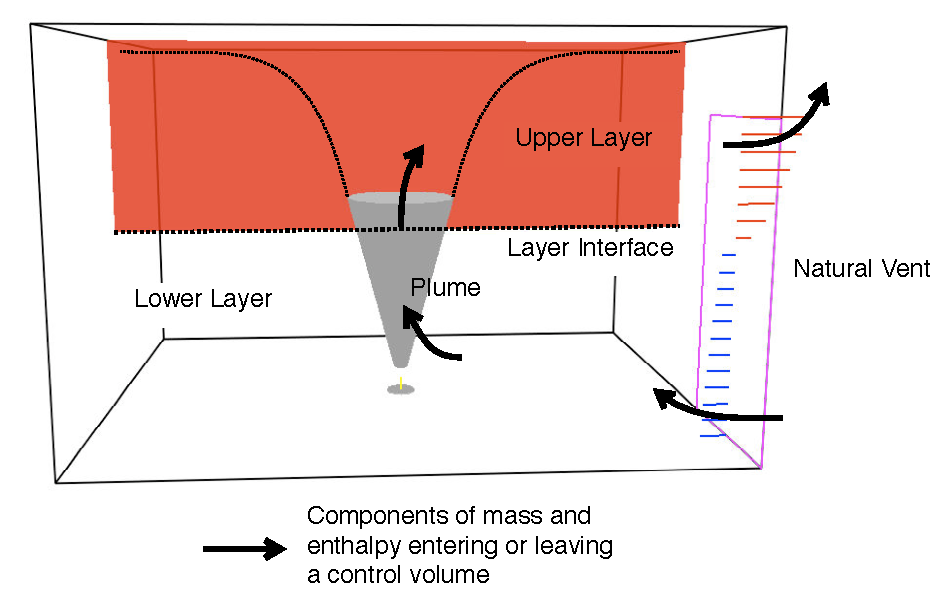
\includegraphics[width=\textwidth]{FIGURES/Theory/Control_Volumes}\\
\end{center}
\caption{Schematic of control volumes in a two-layer zone model.}
 \label{fig:Control_Volumes}
\end{figure}

The fundamental equations start with the conservation of mass. The change of mass in each layer, $i$, is expressed as
\be
   \dbydt{m_i} = \dot m_i  \label{mass_con}
\ee
where $\dm_i$ represents the sum of all mass flow terms, such as plume mass entrainment and ventilation, entering and leaving layer $i$. Conservation of energy takes the form of the first law of thermodynamics, which states that the rate of increase of internal energy plus the rate at which the layer does work by expansion is equal to the rate at which enthalpy is added to the gas:
\be
   \dbydt{(c_v m_i T_i)} +  P \dbydt{V_i} =  \dot h_i \label{eq:first_law}
\ee
The enthalpy source term, $\dot h_i$, consists of the fire's heat release rate, conduction losses to walls, and radiation exchange. The layer temperature and mass are related to the layer volume and compartment pressure via the ideal gas law:
\be
  P \, V_i = m_i \, R \, T_i \label{EoS}
\ee
A system of ordinary differential equations for the compartment pressure, upper layer volume, and layer temperatures can be derived from these three basic principles ( Eqs. \ref{mass_con}-\ref{EoS}):
\begin{eqnarray}
\dbydt{P} &=& \frac{{\gamma-1}}{{V}} \left( \dhl + \dhu \right)  \label{eq1} \\[.1in]
\dbydt{\Vu} &=& \frac{1}{P \gamma} \left( (\gamma-1) \, \dhu - \Vu \dbydt{P} \right) \label{eq2} \\[.1in]
\dbydt{\Tu} &=& \frac{1}{c_p \, m_{\rm u}} \left( \dhu - c_p \, \dmau \, \Tu + \Vu \dbydt{P} \right) \label{eq3} \\[.1in]
\dbydt{\Tl} &=& \frac{1}{c_p \, m_{\rm l}} \left( \dhl - c_p \, \dmau \, \Tl + \Vl \dbydt{P} \right) \label{eq4}
\end{eqnarray}
Equation~(\ref{eq1}) is derived by summing Eq.~(\ref{eq:first_law}) for the upper and lower layer, applying the equation of state~(\ref{EoS}), and noting that the time derivative of the total room volume is zero. Equation~(\ref{eq2}) is derived by rearranging Eq.~(\ref{eq:first_law}) applied to the upper layer and applying the equation of state to replace the internal energy term. Equations~(\ref{eq3}) and (\ref{eq4}) are derived from Eq.~(\ref{eq:first_law}) applied to each layer, along with substitutions of the equation of state and mass conservation equation.

As discussed in Refs.~\cite{Forney:1994} and \cite{Rehm:1992}, Eqs.~(\ref{eq1}) through (\ref{eq4}) are stiff, meaning that the pressure adjusts to changing conditions far more quickly than the other variables. Runge-Kutta methods or predictor-corrector methods such as Adams-Bashforth require prohibitively small time steps in order to track the short time scale phenomena (pressure in our case). Methods that calculate the Jacobian (or at least approximate it) have a much larger stability region for stiff problems and are thus more successful at their solution (see, for example, \cite{Numerical_Recipes}).

\section{Species Transport}

The equation of state, (\ref{EoS}), assumes that the molecular weight of the gaseous mixture throughout the domain is approximately that of air, 29~g/mol. However, CFAST does track the products of combustion and the depletion of oxygen in each zone. At the start of the simulation, the composition of each layer is set to ambient conditions. The initial temperature is specified by the user. The oxygen mass fraction is 23~\% (21~\% volume fraction) and the nitrogen mass fraction is 77~\% (79~\% volume fraction). The mass fraction of water vapor is specified by the user in terms of a relative humidity and the oxygen and nitrogen mass fractions are adjusted accordingly. All other gas species are initially zero.  As fuel is burned, product species are produced in direct proportion to the rate of fuel consumption (the major products of combustion are determined from the specified fuel molecule and the minor species yields are specified by the user). The mass fraction of oxygen can limit the combustion rate as discussed in Section~\ref{section:HRR}). Two special separate species are included in the model -- a generic toxic species and an arbitrary trace species. Both are excluded from the overall mass balance, but they are generated by the fire and transported in a manner identical to the other species.

Each unit mass of a species produced by a fire is carried in the flow to the various rooms and accumulates in the layers. The species mass divided by the layer volume is the mass concentration. Filters can be used in mechanical ventilation systems to remove species. The phenomenon has been implemented in CFAST to remove trace species and soot. It is implemented by modifying the source terms which describe gas flow. See Ref.~\cite{Jones:2008} for an example on the use of filtering.

The calculation of radiation exchange in CFAST also depends in part on the species concentrations calculated by the model (and thus the user inputs for species yields). There are two separate radiation calculations performed by CFAST. The first is for thermal radiation as part of the overall heat transfer calculation, discussed in Section~\ref{sec:Radiation}. The second is for visible light extinction to determine visibility, discussed in Section~\ref{Visibility}.






\chapter{The Fire Plume}
\label{sec:TheFire}

Fires in CFAST are specified by the user in terms of a time-dependent heat release rate (HRR), an effective fuel molecule, and the yields of the products of incomplete combustion like soot and CO. Fires can be specified in multiple compartments and are treated as totally separate entities, with no interaction of the plumes. These fires are generally referred to as ``objects'' and can be ignited at a prescribed time, temperature or heat flux.

CFAST does not include a pyrolysis model to {\em predict}, as opposed to specify, the growth and spread of the fire. Rather, the transient pyrolysis rates for each fire are prescribed by the user. Whereas this approach does not directly calculate the increased pyrolysis due to radiative feedback from the flame or compartment, in theory these effects could be prescribed by the user. For larger fires, this can be an important consideration, and the specification used should reflect the actual conditions as closely as possible.

\section{Combustion Chemistry}

 The HRR of the fire is specified by the user, but it may be constrained by the availability of oxygen in the compartment. The combustion of a hydrocarbon fuel is described by the following single-step reaction:
\begin{eqnarray}
   \mathrm{C_{n_\C}H_{n_H}O_{n_O}N_{n_N}Cl_{n_{Cl}}} &+&  \nu_\OTWO \, \mathrm{O_2}  \rightarrow  \nonumber \\[.1in]
   \nu_\COTWO \, \mathrm{CO_2} &+& \nu_\HTWOO \, \mathrm{H_2O} \; + \; \nu_\CO \, \mathrm{CO} \; + \; \nu_\So \, \mathrm{Soot} \; + \; \nu_\HCl \mathrm{HCl} \; + \; \nu_\HCN \mathrm{HCN} \label{stoich}
\end{eqnarray}
The user specifies the composition of the fuel molecule and the yields of soot and CO, $y_\So$ and $y_\CO$, which are related to their stoichiometric coefficients as follows:
\begin{eqnarray}
   \nu_\So &=& \frac{M_\F}{M_\So} \; y_\So \label{soot_yield} \\[.1in]
   \nu_\CO &=& \frac{M_\F}{M_\CO} \; y_\CO \label{CO_yield}
\end{eqnarray}
Under the assumption that all of the nitrogen and chlorine in the fuel are converted to HCN and HCl, the other stoichiometric coefficients are:
\begin{eqnarray}
  \nu_\COTWO &=& \mathrm{n_\C} - \brackets{\nu_\CO + \nu_\HCN + \nu_\So} \\[.1in]
  \nu_\HTWOO &=& \frac{\mathrm{n_\Hy} - \brackets{\nu_\HCl + \nu_\HCN}}{2} \\[.1in]
  \nu_\OTWO  &=& \nu_\COTWO + \frac{\nu_\HTWOO + \nu_\CO - \mathrm{n_\Oh}}{2} \label{Oxygen_yield} \\[.1in]
  \nu_\HCl   &=& \mathrm{n_{Cl}} \\[.1in]
  \nu_\HCN   &=& \mathrm{n_{N}}
\end{eqnarray}
Note that the nitrogen in the air acts only as a diluent. The yields of hydrogen cyanide and hydrogen chloride are based solely on the composition of the fuel molecule. Finally, a user-specified trace species can be specified to follow the transport that results from fire-induced flow for an arbitrary species. This may be of particular interest for radiological releases \cite{Jones:2008}, but may be useful for any trace amounts released by a fire.



\section{Heat Release Rate}
\label{section:HRR}

As fuel and oxygen are consumed, heat is released and various products of combustion are formed. The heat is released as radiation and convected enthalpy:
\begin{eqnarray}
   \dQr &=& \chir \, \dQ \\[.1in]
   \dQc &=& (1-\chir) \, \dQ \\
\end{eqnarray}
where $\dQ$ is the heat released by the fire. The parameters $\dQr$ and $\dQc$ are the heat released by radiation and convection, respectively, and $\chir$ is the fraction of the fire's heat release rate emitted as radiation.

The user specifies the heat release rate, $\dQ$, as the actual heat released, accounting for combustion efficiency, along with a characteristic base diameter, $D$, which is used in the plume temperature and mass entrainment correlations. The combustion efficiency, $\chia$, is the fraction of the theoretical energy that is actually released during combustion \cite{Hamins:1996}. $\chia$ is a function of fuel type, scale, and vitiation. For small fires, Tewarson provides measured values for specific fuels \cite{Tewarson:2003}. Within CFAST, the user also specifies a radiative fraction which takes a default value of 0.35 ; i.e., 35 \% of the fire's energy is released via radiation.  For specific fuels, the work of Tewarson \cite{Tewarson:2003}, McCaffrey \cite{McCaffrey:1982}, or Koseki \cite{Koseki:1989} is available for reference. The effects of scale, fuel type, vitiation, and combustion efficiency are all important to the radiation released by a fire \cite{Hamins:1991, Hamins:1994}. The typical range for the radiative fraction is from about 0.05 to 0.4. The assumed and constant values for the combustion efficiency and radiative fraction may add uncertainty to the calculated results, so the heat release rate and radiative fraction should be chosen carefully to best model the scenario of interest.

Using the specified heat release rate of the fire, $\dQ$, and a user-specified the heat of combustion, $\Dh$,  the model calculates the pyrolysis rate of fuel, $\dmf$:
\be
   \dmf = \frac{\dQ}{\Dh}
\ee

In the event that the HRR is constrained by the availability of oxygen, it is assumed that the pyrolysis rate does not change. However, only part of the pyrolyzed fuel burns and the HRR becomes:
\be
   \dQ = \min \Big( \dmf \, \Dh \, , \, \dme \, Y_\OTWO \, C_{\rm LOL} \, \DhO \Big)
\ee
where $\dme$ is the entrainment rate, $Y_\OTWO$ is the mass fraction of oxygen in the layer containing the fire, $\DhO$ is the heat of combustion based on oxygen consumption\footnote{The heat of combustion based on oxygen consumption is taken to be 13.1~MJ/kg, representative of typical hydrocarbon fuels~\cite{Huggett:1980}.}, and $C_{\rm LOL}$ (Lower Oxygen Limit) is the smoothing function ranging from 0 to 1:
\be
   C_{\rm LOL} \approx \frac{\tanh \Big( 800 (Y_\OTWO - Y_{\OTWO,{\rm l}}) - 4 \Big) + 1}{2}
\ee
The limiting oxygen mass fraction, $Y_{\OTWO,{\rm l}}$, is 0.1, by default. This value is not a function of temperature.

Any unburned fuel is tracked by the model, and transported to the upper layer via entrainment in the fire plume or to other compartments through any user-specified vents. Unburned fuel may burn in the upper layer or at vents if sufficiently hot and if additional oxygen is available.



\section{Plume Entrainment}

A fire pumps mass and energy from the lower layer into the upper layer. The vertical flow of mass through a horizontal plane at height $z$ above the base of the fire is called the mass entrainment rate, $\dme(z)$. The vertical flow of energy through this horizontal plane is given by $\dQ_{\rm c} + \dme(z) \, c_p \, \Tl$. The empirical correlation for the mass entrainment rate depends on whether the plume is unobstructed, against a wall, or in a corner.

\subsection{Unobstructed Plumes}

The plume mass entrainment, $\dme(z)$, at a height $z$ above the base of the fire is estimated using Heskestad's correlation~\cite{Heskestad:2002}:
\be
   \dme(z) = 0.196 \, \left( \frac{g \, \rho_\infty^2}{c_p \, T_\infty} \right)^{1/3} \, \dQ_{\rm c}^{1/3} \; \brackets{z - z_0}^{5/3} \;
   \left( 1 + \frac{2.9 \, \dQ_{\rm c}^{2/3}}{ \left( \sqrt{g} \, c_p \, \rho_\infty \, T_\infty \right)^{2/3} \, (z-z_0)^{5/3}} \right) \label{mdot_e}
\ee
where $z_0$ is a virtual origin defined as
\be
   \frac{z_0}{D} = -1.02 + 1.4 \, \dQ^{* \, 2/5} \quad ; \quad \dQ^* = \frac{\dQ}{\rho_\infty \, c_p \, T_\infty \, \sqrt{g \, D} \, D^2} \label{virtual_origin}
\ee
Note that the virtual origin is defined in terms of the total heat release rate of the fire, $\dQ$. Equation~(\ref{mdot_e}) is recommended above the mean flame height, $L$. Below the flame height, Heskestad~\cite{Heskestad:2002} recommends the following:
\be
  \dme(z) = \dme(L) \, \frac{z}{L} \quad ; \quad \frac{L}{D} = -1.02 + 3.7 \, \dQ^{* \, 2/5}
\ee
where the mean flame height is defined as the distance from the fuel source to the top of the visible flame where the intermittency is 0.5.  A flame intermittency of 0.5 means that the visible flame is above the mean 50~\% of the time and below the mean 50~\% of the time.

\subsection{Wall and Corner Plumes}

If the fire is located in a corner or against a wall\footnote{CFAST assumes that the fire is in a corner or against a wall {\em only} when the user specifies the {\em exact} coordinates of the corner or wall.}, the unobstructed plume entrainment correlation, Eq.~(\ref{mdot_e}), is modified. For a corner, it is assumed that the fire is mirrored in each wall face, quadrupling the convective HRR, $\dQ_{\rm c}$, and doubling the base diameter, $D$. The entrainment rate, $\dme(z)$, of this hypothetical larger fire is then divided by a factor of 4. The effective entrainment rate is approximately $4^{1/3}/4 \approx 0.40$ of its unobstructed value. Of course, the virtual origin, $z_0$, in Eq.~(\ref{mdot_e}) is affected by the change in effective diameter as well.

If the fire is against a wall, the convective HRR is doubled, the diameter is multiplied by $\sqrt{2}$, and the result of Eq.~(\ref{mdot_e}) is divided by 2. The effective entrainment rate is $2^{1/3}/2 \approx 0.63$ of its unobstructed value.

\subsection{Weak Plumes}

In CFAST, there is a constraint on the mass entrainment rate because the plume can rise only so high for a given HRR.  Early in a fire, the plume may not have sufficient energy to reach the compartment ceiling. Therefore, a limit is placed on the entrainment rate. For the plume to be able to penetrate the hot upper layer, the density of the gas in the plume must be less than the density of the gas in the upper layer. This implies that the upper layer temperature must be less than the plume temperature:
\be
   \Tu < \Tp \approx \frac{ \dQc + \dme \, c_p \, \Tl }{ \dme \, c_p}
\ee
Rearranging terms yields a limit on the mass entrainment:
\be
   \dm_e < \frac{\dQc}{c_p (\Tu - \Tl)}
\ee


\section{Plume Temperature and Velocity}
\label{sec:Plume_Temp_Velocity}

The centerline plume temperature rise, $\Delta T_0(z)$, and velocity, $u_0(z)$, at a height $z$ above the base of the fire is estimated using Heskestad's correlations~\cite{Heskestad:2002}:
\be
   \Delta T_0(z) = \min \left[ 900 \; \mathrm{K} \; , \; 9.1 \, \left( \frac{T_\infty}{g \, c_p^2 \, \rho_\infty^2} \right)^{1/3} \, \dQ_{\rm c}^{2/3} \, (z-z_0)^{-5/3} \right]  \label{plume_temperature}
\ee
\be
   u_0(z) = \min \left[ u_{0,\max} \; , \; 3.4 \, \left( \frac{g}{c_p \, \rho_\infty \, T_\infty} \right)^{1/3} \, \dQ_{\rm c}^{1/3} \, (z-z_0)^{-1/3} \right]  \label{plume_velocity}
\ee
where the virtual origin, $z_0$, is defined in Eq.~(\ref{virtual_origin}). It is assumed that the temperature and velocity decrease following a Gaussian profile about the centerline:
\be
   \Delta T(r,z) = \Delta T_0(z) \, \exp \left[ -\left( \frac{r}{\sigma_{\Delta T}} \right)^2 \right] \quad ; \quad \sigma_{\Delta T} = 0.14 \, \left( \frac{T_0(z)}{T_\infty} \right)^{1/2} \, (z-z_0) \label{plume_temperature2}
\ee
\be
   u(r,z) = u_0(z) \, \exp \left[ -\left( \frac{r}{\sigma_u} \right)^2 \right] \quad ; \quad \sigma_u \approx 1.1 \, \sigma_{\Delta T} \label{plume_velocity2}
\ee
Note that the maximum plume temperature of 900~K is suggested by Heskestad~\cite{Heskestad:2002}. It is also suggested that the maximum centerline plume velocity is reached when the plume temperature rise is 650~K, and is a weak function of the convective HRR:
\be
   u_{0,\max} = 2.2 \left( \frac{g^{2/5}}{T_\infty^{2/5} \, (c_p \, \rho_\infty)^{1/5} } \right) \, \left( 650 \, \dQ_{\rm c} \right)^{1/5}
\ee
Note that if the velocity is expressed in units of m/s and the convective HRR in kW, then $u_{0,\max} \approx 2 \; \dQ_{\rm c}^{1/5}$.

Above the interface between the hot upper layer and the cooler lower layer, the temperature and density of the entrained air is significantly different than that of the lower layer. To account for this, the plume temperature correlation~\cite{Heskestad:2002} is modified for values of $z$ greater than the interface height, $z_{\rm I}$:
\be
   \Delta T_0(z) = 9.1 \, \left( \frac{\Tu}{g \, c_p^2 \, \rho_{\rm u}^2} \right)^{1/3} \, \dQ_{\rm c}^{2/3} \, (z-z_0')^{-5/3}  \quad ; \quad z>z_{\rm I}  \label{plume_temperature_upper}
\ee
where the modified virtual origin is given by:
\be
   z_0' = z_{\rm I} - \left( \frac{\Tu}{\Tl} \right)^{3/5} \, (z_{\rm I}-z_0)  \label{virtual_origin_modified}
\ee
Equations~(\ref{plume_temperature_upper}) and (\ref{virtual_origin_modified}) are obtained by asserting that $\Delta T_0$ is continuous across the layer interface and that $\Tu \rho_{\rm u} \approx \Tl \rho_{\rm l}$.

The mass entrainment correlation, Eq.~(\ref{mdot_e}), is modified the same way above the layer interface.



\chapter{Ventilation}

CFAST models three types of vent flow: natural flow through vertical vents (such as doors or windows),  natural flow through horizontal vents (such as ceiling holes or hatches), and forced flow via mechanical ventilation. Forced flow can occur through either vertical or horizontal vents.


\section{Vertically-Oriented Vents (Doors and Windows)}

Natural flow through windows and doors is governed by the vertical stratification of the pressure difference across the opening~\cite{Emmons:SFPE}. The mass flow is calculated by dividing the opening into discrete horizontal segments, each of which is bounded by the top or bottom of the opening, the zone interface of either compartment, or the neutral plane, which is where the velocity changes direction. This is shown schematically in Fig.~\ref{fig:Flow_Patterns}.

\begin{figure}[t]
\setlength{\unitlength}{1in}
\begin{picture}(6.5,4)
\thicklines
\put(0,0){\line(1,0){6.5}}
\put(0,4){\line(1,0){6.5}}
\put(3.25,4){\line(0,-1){1}}
\thinlines
\put(0,1.5){\line(1,0){3.25}}
\put(3.25,2.5){\line(1,0){3.25}}
\put(0,2.0){\line(1,0){6.5}}
\put(3.5,0.75){\vector(-1,0){0.5}}
\qbezier(3.5,1.75)(3.25,1.75)(3.0,1.5)
\put(3.0,1.5){\vector(-1,-1){0.2}}
\qbezier(3,2.25)(3.25,2.25)(3.5,2.5)
\put(3.5,2.5){\vector(1,1){0.2}}
\put(3,2.75){\vector(1,0){0.5}}

\put(1.625,3.8){\makebox(0,0){Compartment 1}}
\put(4.875,3.8){\makebox(0,0){Compartment 2}}
\put(6,1.85){\makebox(0,0){Neutral Plane}}
\put(5.95,2.35){\makebox(0,0){Layer Interface}}
\put(0,1.35){Layer Interface}
\put(3.75,0.75){\makebox(0,0){$\dm_{\rm l \to l}$}}
\put(3.75,1.75){\makebox(0,0){$\dm_{\rm l \to u}$}}
\put(2.75,2.25){\makebox(0,0){$\dm_{\rm u \to l}$}}
\put(2.75,2.75){\makebox(0,0){$\dm_{\rm u \to u}$}}

\end{picture}
\caption{Flow patterns for horizontal flow through a vertical vent.}
\label{fig:Flow_Patterns}
\end{figure}

Let $z=b$ and $z=t$ denote the height of the bottom and top of the segment, and $\Delta P_b$ and $\Delta P_t$ denote the pressure differences at these heights.  Because a given segment is either completely above or completely below the neutral plane, the two pressure differences will have the same sign. The mass flow through the segment can then be computed by integrating Bernoulli's equation from $b$ to $t$:
\begin{eqnarray}
\dm &=& \int_b^t C \sqrt{2 \rho \, \Delta P(z)} \, w \; \rd z  \\[.1in]
    &=& C\sqrt{2\rho} \, w \int_b^t\sqrt{\frac{|(t-z) \, \Delta P_b + (z-b) \, \Delta P_t|}{t-b}} \; \rd z \\[.1in]
    &=& \frac{2}{3} \, C \sqrt{2\rho} \, w \, (t-b)\frac{|\Delta P_t|^{3/2}-|\Delta P_b|^{3/2}}{|\Delta P_t|-|\Delta P_b|}
\label{eq:massflowone}
\end{eqnarray}
Here, $C$ is the orifice coefficient taken to be 0.7~\cite{Steckler_Coefficients}, $\rho$ is the gas density of the upwind compartment, $w$ is the width of the opening, and $\Delta P(z)$ is the pressure across the interface at elevation $z$. Note the use of the integral formula
\begin{eqnarray}
\int \sqrt{A+Bz} \; \rd z = \frac{2}{3B}(A+Bz)^{3/2}+\mbox{constant}
\end{eqnarray}
where $A=(|t\,\Delta P_t|-b\,|\Delta P_b|)/(t-b)$ and $B=(|\Delta P_t|-|\Delta P_b|)/(t-b)$. Equation \ref{eq:massflowone} can be written:
\be
   \dm = \frac{2}{3} C \sqrt{2 \rho} \, w \, (t-b)  \frac{|\Delta P_t|+\sqrt{|\Delta P_t \,\Delta P_b|}+|\Delta P_b|}{\sqrt{|\Delta P_t|}+\sqrt{|\Delta P_b|} }
\ee
This is the way it is written in Ref.~\cite{Emmons:SFPE}.

Figure~\ref{fig:Flow_Patterns} indicates schematically how the various mass flows through the opening are distributed. For the flow originating in the upper layer of the upstream compartment flowing into the upper layer of the downstream compartment, $\dm_{\rm u \to u}$, or the flow from the lower layer to the lower layer, $\dm_{\rm l \to l}$, the mass is applied directly to the downstream layer.

The mass flow from the upper layer of the upstream compartment to the lower layer of the downstream, $\dm_{\rm u \to l}$, is assumed to rise into the upper layer via a spill plume. The enthalpy flow rate of the plume is:
\be
   \doh_{\rm u \to l} = c_p \brackets{T_{\rm u,1}-T_{\rm l,2}} \, \dm_{\rm u \to l}
\ee
Assuming that $T_{\rm u,1} > T_{\rm l,2}$, the mass entrainment of the spill plume is given by Poreh {\em et al.}~\cite{Poreh:1998}:
\be
   \dm_{\rm e,p} = \dm_{\rm u \to l} \, + \, C_{\rm m} \, \left( \frac{T_{\rm l,2}}{T_{\rm u,1}} \right)^{2/3} \, \left( \frac{ g \, \rho_{\rm l,2}^2}{c_p \, T_{\rm l,2}} \right)^{1/3} \, \doh_{\rm u \to l}^{1/3} \; w^{2/3} \;
   (z_{\rm I}-z_{\rm N})
\ee
where $C_{\rm m}$ is an empirical constant equal to 0.44, $w$ is the width of the opening, $z_{\rm I}$ is the height of the layer interface, and $z_{\rm N}$ is the height of the neutral plane. Suggested values for $C_{\rm m}$ vary between 0.44 and 0.66, all of which were determined empirically in a number of different experimental configurations.

For the mass flow leaving the lower layer of the upstream compartment and entering the upper layer of the downstream compartment, $\dm_{\rm l \to u}$, the shear flow causes vortex shedding that entrains upper layer gas and deposits it in the lower layer. It is assumed that the incoming cold plume behaves like the inverse of the usual door jet between adjacent hot layers; forming a descending plume.  The same equations are used to calculate this inverse plume as are used for the upright door mixing, above.

\section{Horizontally-Oriented Vents (Floor and Ceiling Vents)}

Flow through a ceiling or floor vent is governed by both pressure and density differences. The simplest form is uni-directional flow driven primarily by a relatively large pressure difference. When the pressure difference is relatively small, the density difference, where hot gas underlies colder gas, can lead to bi-directional flow where the gas in the lower compartment rises into the upper compartment and {\em vice versa}.  This situation might arise in a real fire if the room of origin suddenly has a hole open up in the ceiling.

Cooper's algorithm~\cite{Cooper:1989, Cooper:1990, Cooper:1995} is used for computing mass flow through ceiling and floor vents:
\be
   \dm = 0.1 \brackets{\frac{g \, \Delta \rho \, A_{\rm v}^{5/2}}{\rho_{\rm avg}}} \brackets{1 - \frac{2 \, A_{\rm v}^2 \, \Delta P}{S^2 \, g \, \Delta \rho \, D^5}}
\ee
where $D = 2 \sqrt{A_{\rm v} / \pi}$ and $S$ is 0.754 for round or 0.942 for square openings, respectively. For each layer on either side of the vent, there are two values of the mass flow, $\dm_{\rm in}$ and $\dm_{\rm out}$. These terms are symmetric: the outgoing flow from one compartment is the incoming flow to the other. The corresponding enthalpy flows are determined from the relative size and temperature of the lower and upper layers:
\begin{eqnarray}
  \doh_{\rm in} &=& c_p \, \dmu \, \Tu + c_p \, \dml \, \Tl \\[0.1in]
  \dmu &=& \dm_{\rm in} \, \frac{\Vu}{V} \\[0.1in]
  \dml &=& \dm_{\rm in} \, \frac{\Vl}{V}
\end{eqnarray}
The mass and energy are then deposited into the upper or lower layer of the receiving compartment based on the effective temperature of the incoming flow. If the temperature of the incoming flow is higher than the temperature of the lower layer of the receiving compartment, then the flow is deposited into the upper layer. Otherwise, it is deposited into the lower layer of the receiving compartment. This is similar to the idea of using a virtual plume for a doorway flow.


\section{Forced Flow}

CFAST models mechanical ventilation in terms of user-specified volume flows at various points in the compartment. The model does not include duct work or fan curves. These equations are high-order, non-linear and in some cases ill-posed, which caused a great deal of difficulty in reaching a numerical solution.

The flow through mechanical vents can be filtered. Filtering affects particulates such as smoke and the trace species. Filtering can be turned on at any time. Effectiveness is from 0~\% (no effect) to 100~\% which completely blocks the flow of these two species.





\chapter{Heat Transfer}

This section discusses thermal radiation, convection, and conduction, the three mechanisms by which heat is transferred between the gas layers and the enclosing compartment walls. Hot gases exchange heat with solid surfaces via convection and radiation. Heat is transferred through solids via conduction. Different material properties can be used for the ceiling, floor, and walls of each compartment (although all the walls of a compartment must be the same).  Additionally, each surface can be composed of up to three distinct layers.  This allows the user to deal naturally with the actual building construction.  Material thermophysical properties are assumed to be constant. Radiative transfer occurs among the fire(s), gas layers and compartment surfaces (ceiling, walls and floor).  This transfer is a function of the temperature differences and the emissivity of the gas layers as well as the compartment surfaces.  Typical surface emissivity values only vary over a small range.  For the gas layers, however, the emissivity is a function of the concentration of species which are strong radiators, predominately smoke particulates, carbon dioxide, and water.

\section{Radiation}
\label{sec:Radiation}

Radiation heat transfer is calculated between the ceiling, floor, wall layers, and fire, with the inclusion of emission and absorption by the hot gas layer~\cite{Forney_radiation}. The following assumptions are made:
\begin{itemize}
\item Each gas layer and each wall segment is assumed to be at a uniform temperature.
\item The wall and gas layer temperatures are assumed to change slowly over the duration of the time step of the governing equations.
\item The fire is assumed to radiate uniformly in all directions emitting a fraction, $\chi_{\rm r}$, of the total heat release rate.  This radiation is assumed to originate from a single point.  Radiation feedback to the fire and radiation from the plume is not modeled in the radiation exchange algorithm.
\item The radiation emitted is assumed to be diffuse and gray.  In other words, the radiant fluxes emitted are independent of direction and wavelength. At a solid surface, the emittance, $\epsilon$, absorptance, $\alpha$, and reflectance, $\rho$, are related via $\epsilon = \alpha = 1 - \rho$. In the gas phase, the emittance, $\epsilon$, absorptance, $\alpha$, and transmittance, $\tau$, are related via $\epsilon = \alpha = 1 - \tau$.
\item Rooms or compartments are assumed to be rectangular boxes.  Each wall is either perpendicular or parallel to every other wall.  Radiation transfer through vent openings is lost from the room.
\end{itemize}
The compartment lining is divided into four parts: the ceiling, the floor, and the wall sections above and below the layer interface. The net radiative heat flux at surface~$k$, $\dq_k''$, is found by solving the simplified radiation transport equation given by Eq.~(17-20) in Siegel and Howell~\cite{SiegelandHowell:1981}:
\be
   \frac{\dq_k''}{\epsilon_k} - \displaystyle\sum_{j=1}^N \frac{1 - \epsilon_j}{\epsilon_j} \, \dq_j'' \, F_{k-j} \, \tau_{k-j} = \sigma T_k^4 - \displaystyle\sum_{j=1}^N \brackets{\sigma T_j^4 \, F_{k-j} \, \tau_{k-j}} - c_k \label{RTE}
\ee
where $F_{k-j}$ is the configuration factor (fraction of radiant energy emitted by surface $j$ that is intercepted by surface $k$), $\tau_{k-j}$ is the transmittance, $\sigma$ is the Stefan-Boltzman constant, $\epsilon_k$ is the emissivity, $A_k$ is the area, and $T_k$ is the temperature of surface $k$. The radiation from the hot gas layer and the fire is included in the last term:
\be
   c_k = \epsilon_{\rm u} \, F_{{\rm u}-k} \, \sigma \, \Tu^4 + \frac{\omega_{{\rm f}-k}}{4 \pi} \frac{\chi_{\rm r} \, \dQ}{A_k}  \label{ckeq}
\ee
where $\epsilon_{\rm u}$ is the emittance (absorptance) of the upper layer, $F_{{\rm u}-k}$ is the view factor between the upper layer and solid surface, $\omega_{{\rm f}-k}$ is the solid angle between the fire and wall\footnote{Note that as the area of surface $k$ shrinks to zero, $\omega_{{\rm f}-k}/A_k \to 1/R^2$, yielding the classic point source radiation model}, and $\dQ$ is the heat release rate of the fire. If the solid surface, $k$, is the floor or the lower wall, the view factor refers to the layer interface. If the solid surface is the upper wall or ceiling, the view factor is 1.

Reference~\cite{Forney_radiation} describes the solution of Eq.~\ref{RTE}.


\subsection{Configuration Factors}

The configuration factor, $F_{1-2}$, is the fraction of radiant energy emitted by surface 1 that is intercepted by  surface 2, and is calculated:
\be
   F_{1-2} = \frac{1}{A_1} \int_{A_1} \int_{A_2} \frac{\cos \theta_1 \, \cos \theta_2}{\pi L^2} \, dA_2 \, dA_1 \label{eq:config_factor}
\ee
where $L$ is the distance along the line of integration,  $\theta_1$ and $\theta_2$ are the angles for surface 1 and 2 between the respective normal vectors and the line of integration, and $A_1$ and $A_2$ are the areas of the two surfaces.  These terms are illustrated in Fig.~\ref{fig:Rad_Config_Factor}.
\begin{figure}
\begin{center}
\includegraphics[width=3.0in]{FIGURES/Theory/Radiation_Config_Factor}\\
\end{center}
\caption{Setup for a configuration factor calculation between two arbitrarily oriented finite areas.}
 \label{fig:Rad_Config_Factor}
\end{figure}
There are two types of configuration factors in CFAST. First, consider two rectangles perpendicular to each other having a common edge of the same length, $l$. The dimension of the source rectangle is $l \times w$ and the target rectangle is $l \times h$. The configuration factor from source to target is:
\begin{eqnarray}
\lefteqn{F_{1-2} = \frac{1}{\pi \, W} \left[ W \, \tan^{-1} \frac{1}{W} + H \, \tan^{-1} \frac{1}{H} - \sqrt{H^2+W^2} \, \tan^{-1} \frac{1}{\sqrt{H^2+W^2}} + \right.}  \nonumber \\[.1in]
& &   \left. \frac{1}{4} \, \ln \left\{ \frac{(1+W^2)(1+H^2)}{1+W^2+H^2} \, \left( \frac{W^2(1+W^2+H^2)}{(1+W^2)(W^2+H^2)} \right)^{W^2} \left( \frac{H^2(1+W^2+H^2)}{(1+H^2)(W^2+H^2)} \right)^{H^2} \right\} \right]
\end{eqnarray}
where $H=h/l$ and $W=w/l$.

Next, consider two identical, parallel, directly opposed rectangles. The dimension of the rectangles is $a \times b$ and the separation distance is $c$. The configuration factor is:
\begin{eqnarray}
\lefteqn{F_{1-2} = \frac{2}{\pi \, X \, Y} \left\{ \ln \left[ \frac{(1+X^2)(1+Y^2)}{1+X^2+Y^2} \right]^{1/2} + X \sqrt{1+Y^2} \, \tan^{-1} \frac{X}{\sqrt{1+Y^2}} + \right.} \nonumber \\[.1in]
& & \left. Y \sqrt{1+X^2} \, \tan^{-1} \frac{Y}{\sqrt{1+X^2}} - X \, \tan^{-1} X - Y\, \tan^{-1} Y \right\}
\end{eqnarray}
where $X=a/c$ and $Y=b/c$. These formulae are found in Appendix~C of Ref.~\cite{SiegelandHowell:1981}.

Next, the normalized solid angle, $\omega_{\rm f-k}$, in Eq.~(\ref{ckeq}) is computed. First, place a sphere of radius $r$ tangent to a rectangle of dimension $x \times y$ such that the point of tangency is the corner of the rectangle. The normalized solid angle formed by the center of the sphere and the edges of the rectangle is given by:
\be
   \omega(x,y;r) = \frac{1}{4\pi} \left[ \sin^{-1} \left( \frac{A \, y}{\sqrt{y^2+r^2}} \right) + \sin^{-1} \left( \frac{A \, x}{\sqrt{x^2+r^2}} \right) - \frac{\pi}{2} \right] \quad ; \quad A=\sqrt{1+\frac{r^2}{x^2+y^2}}
\ee
Suppose now that the radiation of a fire is assumed to emanate from a point a distance $r$ above the floor whose dimension is $L \times W$. Suppose also that the floor is divided into four quadrants based on the location of the fire. The dimensions are partitioned $L=L_1+L_2$ and $W=W_1+W_2$. The normalized solid angle between the point source fire, f, and the floor, fl, is:
\be
   \omega_{\rm f-fl} = \sum_{j=1}^2 \sum_{i=1}^2 \omega(L_i,W_j;r)
\ee

\subsection{Transmittance and Absorptance}

The transmittance is the fraction of radiant energy that will pass through a volume filled with an absorbing medium. It is usually expressed in the form:
\be
   \tau = {\rm e}^{-a L}
\ee
where $a$ is the absorption coefficient and $L$ is the path length. The absorptance is the fraction of radiant energy absorbed by that volume. For a gray gas, $\alpha + \tau = 1$.

In general, the transmittance and absorptance are functions of wavelength. This is an important factor to consider for the major gaseous products, $\textnormal{CO}_2$  and $\textnormal{H}_2 \textnormal{O}$. However, soot has a continuous absorption spectrum that allows the transmittance and absorptance to be approximated as ``gray'' \cite{SiegelandHowell:1981} across the entire spectrum. The total transmittance over a path length $L$ through a volume of combustion products is taken as the product of the transmittance of the soot and major gas phase products:
\be
   \tau = e^{-a_{\rm s}L} \brackets{1 - \alpha_{\rm H_2O} - 0.5 \, \alpha_{\rm CO_2}}
\ee
The factor of 0.5 applied to the absorptance of CO$_2$ accounts for the overlap of the wavelength bands of the two gases. Tien~et~al.~\cite{Tien:2002} suggest that the absorption coefficient for soot may be approximated as $a_{\rm s} = k f_v T$ where $k$ is a constant that depends on the optical properties of the soot particles, $f_v$ is the soot volume fraction, and $T$ is the (absolute) temperature. Values of $k$ have been found to be about constant for a wide range of fuels~\cite{Tien:1978}.

Absorptance data for $\textnormal{H}_2 \textnormal{O}$ and $\textnormal{CO}_2$ are reported in Ref.~\cite{Edwards:1985}. For each gas, these data are tabulated and implemented as a two-dimensional array based on temperature and gas concentration.

The effective path length, $L$, is calculated between the center-points of the exchanging surfaces ({\em i.e.}, from the center height of a fire to the center of a wall surface or between the center points of two compartment surfaces). Path lengths are calculated separately for the upper and lower layers in a compartment.




\section{Convection}

The transfer of heat between the gas and solid surfaces is handled slightly differently at the ceiling, floor and walls, due to the difference in orientation and the presence of a relatively thin hot flow near the ceiling known as the ceiling jet. The following two sections describe how the convective heat transfer is done for these different surfaces.

\subsection{Walls and Floor}

In general, the convective heat flux to a solid surface is given by:
\be
   \dqc'' = h \, \brackets{\Tg - \Ts}  \label{convective_heat_flux}
\ee
The convective heat transfer coefficient, $h$, is a function of the gas properties, temperature, and velocity. In CFAST, simple correlations for natural convection are used, since the gas velocity is unknown:
\be
   h = C {|\Tg - \Ts|}^{1/3}
\ee
where $C$ is an empirical coefficient (1.52 for the floor and ceiling (in the absence of a ceiling jet) and 1.31 for the walls~\cite{Holman:1990}), $\Tg$ is the average gas layer temperature adjacent to the surface, and $\Ts$ is the surface temperature.

\subsection{Ceiling}

During the early stage of a fire before a hot gas layer has formed, the convective heat transfer to the ceiling is governed by the temperature and velocity of the ceiling jet. Alpert's chapter in the {\em SFPE Handbook}~\cite{Alpert:SFPE} presents an empirical correlation for the convective heat flux from the ceiling jet to a relatively cool surface:
\be
   \dqc'' = 1.323 \, f \, \frac{\dQ_{\rm c}}{H^2} \, \left( \frac{r}{H} \right)^{-1.36}  \label{eq:cjflux}
\ee
where $f$ is a friction factor estimated to be 0.03, $r$ is the radial distance to the plume centerline, $H$ is the ceiling height, and $\dQ_{\rm c}$ is the convective fraction of the heat release rate. The average convective heat flux to the ceiling can be obtained by integrating this expression over the entire ceiling:
\be
   \dq_{\rm c,avg}'' = \frac{1}{LW} \int_0^{2\pi} \int_0^R \dqc'' \, r \, dr \, d\theta = \frac{0.27 \, \dQ_{\rm c}}{(LW)^{0.68} \, H^{0.64}} \label{eq:cjfluxavg}
\ee
Note that the integration is carried out over a circle whose area, $\pi R^2$, is taken as equal to the area of the ceiling, $LW$.

Equation~(\ref{eq:cjfluxavg}) applies to the early stage of the fire; thus, a modified heat transfer coefficient is used so that there is a transition from the early to later stages when a layer has formed:
\be
   h = \max \left( \frac{\dq_{\rm c,avg}''}{\Tu-\Ts} \, , \, C {|\Tu - \Ts|}^{1/3} \right)
\ee
Here, $\Tu$ is the average temperature of the upper layer and $\Ts$ is the ceiling surface temperature. Notice that the rightmost term is simply the correlation used for the walls and floor.



\section{Heat Conduction within Solid Walls or Targets}

The heat conduction equation is solved in the direction normal to solid target or wall surfaces using non-uniformly spaced nodes and a second-order accurate central difference scheme for the spatial derivatives and a semi-implicit time marching scheme. At each time step, the internal solid temperatures are updated in time until the net convective and radiative heat flux striking the wall equals with the heat flux into the solid~\cite{Moss:1992}:
\be
   \dq'' \equiv \dqr'' + \dqc'' = -k \, \frac{dT}{dx} \Big|_{x=0}
\ee
where $k$ is the thermal conductivity of the solid.  This solution strategy requires a differential algebraic equation (DAE) solver that can simultaneously solve both differential and algebraic equations.  With this method, only one or two extra equations are required per wall segment (two if both the interior and exterior wall segment surface temperatures are computed).  This solution strategy is more efficient than the method of lines since fewer equations need to be solved. Conduction is then coupled to the gas phase energy exchange.

A non-uniform array of internal nodes is used to capture steep gradients in temperature near the surface. Define a penetration depth of
\be
   x_p = 2 \sqrt{\alpha \, t_{\rm end}} \; \hbox{erfc}^{-1} \brackets{0.05}
\ee
where $\hbox{erfc}^{-1}$ denotes the inverse of the complementary error function. The value $x_p$ is the location in a semi-infinite wall where the temperature rise is 5~\% after $t_{\rm end}$ seconds. Eighty percent of the nodes are placed on the interior side of $x_p$ and the remaining 20~\% are placed on the exterior side.

The heat conduction equation normal to the solid surface is:
\be \frac{\partial T}{\partial t} = \frac{k}{\rho c}\frac{\partial^2 T}{\partial x^2}
\label{eq:Target_PDE} \ee
where $k$, $\rho$ and $c$ are the thermal conductivity, density and heat capacity of the target. At the surface, $x=0$, the boundary condition is:
\be
   \dq''=-k\frac{dT}{dx} \label{eq:Target_Fourier}
\ee
where $\dq''$ is the net convective and radiative heat flux.

\newcommand{\Dt}{\Delta t}
\newcommand{\Dr}{\Delta r}
\newcommand{\Tipo}{T_{i+1}^{n+1}}
\newcommand{\Ti}{T_{i}^{n+1}}
\newcommand{\Timo}{T_{i-1}^{n+1}}

The 1-D heat conduction equation can be solved in either Cartesian or cylindrical coordinates. The solution methodology shall be presented for cylindrical coordinates:
\be
  \frac{\partial T}{\partial t} = \frac{k}{\rho c} \frac{1}{r} \frac{\partial}{\partial r} \left( r \frac{\partial T}{\partial r} \right)
\ee
Dividing the cylinder into $N$ uniformly spaced concentric control volumes, this equation can be written in discretized form:
\begin{eqnarray}
\Ti-T_i^n&=& \frac{\Dt}{\Dr} \frac{k}{\rho c}
\left[
\left(\frac{\Tipo-\Ti}{\Dr}\right)
\frac{r_i}{r_{i-1/2}}-
\left(\frac{\Ti-\Timo}{\Dr}\right)
\frac{r_{i-1}}{r_{i-1/2}}
\right]
\nonumber\\[0.2in]
&=&\frac{\Dt \, \alpha}{\Dr^2}
\left[
\left(\Tipo-\Ti\right)
\left(\frac{i}{i-0.5}\right)-
\left(\Ti-\Timo\right)
\left(\frac{i-1}{i-0.5}\right)
\right]
\label{eq:cylheat6}
\end{eqnarray}
where $\alpha=k/(\rho c)$. Defining $C_i$ and $D_i$ as
\be
C_i = \frac{\alpha\Dt}{\Dr^2}\left(\frac{i-1}{i-0.5}\right) \quad ; \quad D_i = \frac{\alpha\Dt}{\Dr^2}\left(\frac{i}{i-0.5}\right)
\ee
Eq.~(\ref{eq:cylheat6}) can be written:
\be
-C_i \, \Timo + \left( 1+2\frac{\alpha\Dt}{\Dr^2} \right) \, \Ti - D_i \, \Tipo = T_i^n  \quad \quad i=1...N-1
\label{eq:cylheat8}
\ee
The boundary condition is applied at control volume $N$:
\begin{eqnarray*}
T_N^{n+1}-T_N^n=\frac{\alpha\Dt}{\Dr^2}
\left[\frac{\Dr \, \dq''}{k} \frac{N}{N-0.5} -(T_N^{n+1}-T_{N-1}^{n+1}) \frac{N-1}{N-0.5} \right]
\end{eqnarray*}
or
\be
-C_N \, T_{N-1}^{n+1}+ \left( 1+C_N \right) T_N^{n+1} = T_N^n+D_N\frac{\Dr}{k} \dq''
\label{eq:cylheat10}
\ee
The internal temperature profile, $T_i$, is then obtained with a tri-diagonal linear solver.




\section{Coupling the Gas and Solid Phase Calculations}

To illustrate the method, consider a one room case with one active wall.  There are four gas phase equations (pressure, upper layer volume, upper and lower layer temperatures) and one wall temperature equation.  Implementation of the gradient matching method requires that storage be allocated for the temperature profiles at the current time step, $t$, and at the next time step, $t + \Delta t$.  Given the profile at time $t$ and values for the five unknowns at time $t + \Delta t$ (initial guess by the solver), the temperature profile is advanced from time $t$ to $t + \Delta t$.  The temperature gradient at the wall surface is computed followed by the residuals for the five equations.  The DAE solver adjusts the solution variables and the time step until the residuals for all the equations are below an error tolerance.  Once the solver has completed the step, the array storing the temperature profile for the previous time is updated, and the DAE solver is ready to take its next step.

Heat transfer between connected compartments is modeled by merging the back surfaces of the connected ceiling and floor of the compartments or the back wall surfaces of the connected horizontal compartments.  A heat conduction problem is solved for the merged walls using a temperature boundary condition for both the near and far wall.  As before, temperatures are determined by the DAE solver so that the heat flux striking the wall surface (both interior and exterior) is consistent with the temperature gradient at that surface.

For horizontal heat transfer between compartments, the connections may be between partial wall surfaces, expressed as a fraction of the wall surface. CFAST first estimates conduction fractions analogous to radiation configuration factors. For example, if only one half of the rear wall in one compartment is adjacent to the front wall in a second compartment, the conduction fraction between the two compartments is 0.5. Once these fractions are determined, an average flux, $\dq_{\rm avg}''$, is calculated using
\be
   \dq_{\rm avg}'' = \sum_{\rm walls} \, F_{i-j} \, \dq_j''
\ee
where $F_{ij}$ is the fraction of flux from wall $i$ that contributes to wall $j$, $\dq_j''$ is the flux striking wall $j$.



\chapter{Fire Protection Devices}



\section{Sprinkler and Heat Detector Activation}

The link temperature of a sprinkler or heat detector is modeled using the differential equation~\cite{Schifiliti:2002}:
\be
   \frac{d \TL}{dt} = \frac{\sqrt{v}}{\rm RTI} \brackets{\Tg - \TL}  \label{eq:RTI}
\ee
where $\TL$ and $\Tg$ are the link and gas temperatures, $v$ is the gas speed, and RTI (Response Time Index) is a measure of the sensor's thermal inertia. The gas temperature and speed are obtained from the plume algorithm (Section~\ref{sec:Plume_Temp_Velocity}) and the ceiling jet algorithm, described below. Rooms without fires do not have ceiling jets, in which case the upper layer temperature is used, along with a fixed speed of 0.1~m/s. This value is simply an order of magnitude estimate. The link and gas temperatures and the speed are functions of time; the RTI is a constant for a given detector type. The detector equation is solved numerically using the semi-implicit updating scheme:
\be
   \frac{\TL^{n+1}-\TL^n}{\Delta t} = \frac{1}{2} \left( \frac{\sqrt{v^n}}{\rm RTI} \brackets{\Tg^n - \TL^n}  + \frac{\sqrt{v^{n+1}}}{\rm RTI} \brackets{\Tg^{n+1} - \TL^{n+1}}  \right) \label{eq:RTI_rewritten}
\ee
where the superscript $n$ denotes the value at the current time, and $\Delta t$ is the time step.

The temperature and velocity just below the ceiling is typically greater than that of the upper layer due to the presence of a ceiling jet. From the work of Alpert and Heskestad~\cite{Alpert:SFPE}, the temperature of an unconfined ceiling jet is given by:

\be
   T_{\rm cj}(r) - T_\infty = T_\infty \, \dQ^{* \, 2/3}_H \, \left\{ \begin{array}{l@{\quad}l}
   6.3                                       & ; \quad r/H\le 0.2 \\[0.1in]
   \left( 0.225 + 0.27 \, r/H \right)^{-4/3} & ; \quad 0.2 < r/H < 4.0
    \end{array} \right.
\ee
To be consistent with the calculated plume temperature, this is adjusted so that the calculated plume and ceiling jet temperatures are the same for $r/H \le 0.2$:
\be
   T_{\rm cj}(r) - T_\infty = \left\{ \begin{array}{l@{\quad}l}
   \Delta T_0(H)                                                       & ; \quad r/H\le 0.2 \\[0.1in]
   0.182 \; \Delta T_0(H) \, \left( 0.225 + 0.27 \, r/H \right)^{-4/3} & ; \quad 0.2 < r/H < 4.0
    \end{array} \right. \label{Tcj}
\ee
where $\Delta T_0(H)$ is the calculated centerline plume temperature rise at the compartment ceiling from  Eq.~\ref{plume_temperature} and the constant 0.182 is $\left({0.225 + 0.27 \cdot 0.2} \right)^{4/3}$.

The radial velocity is given by:
\be
   v_{\rm cj}(r) = \sqrt{g \, H} \, \dQ^{* \, 1/3}_H \left\{ \begin{array}{l@{\quad}l}
   3.61                               & ; \quad r/H \le 0.17 \\[0.1in]
   1.06 \, \left( r/H \right)^{-0.69} & ; \quad 0.17 < r/H < 4.0 \end{array} \right. \label{Ucj}
\ee
where the heat release rate of the fire is contained within the non-dimensional expression:
\be
\dQ^*_H = \frac{\dQ}{\rho_\infty \, c_p \, T_\infty \, \sqrt{g} \, H^{5/2}}  \label{QsH}
\ee
To account for the presence of an upper layer, the background temperature, $T_\infty$, in Eq.~(\ref{Tcj}) is replaced with the upper layer temperature, $\Tu$. No adjustment need be made to Eq.~(\ref{QsH}) because $\rho_\infty \, T_\infty$ is assumed constant.

An estimate of the ceiling jet thickness, $\delta$, where the excess temperature drops to 1/e of its maximum value, is given by Motevalli and Marks~\cite{Alpert:SFPE}:
\be
   \frac{\delta}{H} = 0.112 \, \left[ 1-\exp\left( -2.24 \, \frac{r}{H} \right) \right] \quad ; \quad 0.26 \le \frac{r}{H} \le 2.0
\ee
If the detector or sprinkler is below the ceiling jet layer or in a compartment without a fire, the upper layer temperature and a default speed of 0.1~m/s. The basis of this last value is simply an order of magnitude estimate.

If the sprinkler or detector is in a corridor of width, $W$, Delichatsios~\cite{Alpert:SFPE} suggests the following alternative to the ceiling jet correlation, Eqs.~(\ref{Tcj}) and (\ref{Ucj}). For a given distance down the corridor, $x$, from the plume centerline, the excess temperature and velocity are estimated as:
\begin{eqnarray}
   \frac{\Delta T_{\rm cj}(x)}{\Delta \Tp} &=& 0.37 \, \left( \frac{H}{W} \right)^{1/3} \, \exp \left[ -0.16 \, \left( \frac{x}{H} \right) \left( \frac{W}{H} \right)^{1/3} \right]  \\[0.1in]
   v_{\rm cj}(x) &=& 0.114 \, \sqrt{H \, \Delta T_{\rm cj}(x) } \, \left( \frac{H}{W} \right)^{1/6}
\end{eqnarray}
where $\Delta \Tp$ is the excess plume temperature at the ceiling. This correlation is applicable once the plume has reached the full width of the corridor and the ceiling jet flow is parallel to the corridor walls so that $x>W/2$. For $x<W/2$, the normal correlations apply.


\section{Visibility}
\label{Visibility}

The visibility calculation depends solely on the soot concentration. Soot production is specified by the user in terms of a yield. Soot is transported like all other gas species and its concentration is used in the optical density calculation. The optical density is given by the expression:
\be
   D = \frac{K_m \, m_{\rm s}'''}{\ln \, 10}
\ee
where $m_{\rm s}'''$ is the mass of soot per unit volume and $K_m$ is the specific extinction coefficient. The default value is 8700~m$^2$/kg based on the recommendation of Mulholland~\cite{Mulholland:SFPE}.

\section{Smoke Detection}

CFAST does not contain an algorithm that accounts for the time delay owing to smoke transport from the fire to the detector location, nor to the penetration of smoke into the detector chamber itself. Instead, CFAST treats a smoke detector as a very sensitive heat detector with an activation temperature rise of 5~$^\circ$C and RTI of 5~(m$\cdot$s)$^{1/2}$. The temperature rise estimate is based on a study performed by Bukowski and Averill~\cite{Bukowski:1998}. The RTI is not based on experiment; it simply provides a slight time delay in activation.

Users are cautioned that this model is very crude and the uncertainty in its predictions are substantial. Consult the CFAST Validation Guide for more details on its validation.


\section{Fire Suppression} \label{sec:suppression}

Fire suppression by water is predicted using a simple empirical model developed by Madrzykowski \cite{Madrzykowski:1992} and Evans~\cite{Evans:1993}. After activation of the sprinkler, $t > t_{\rm act}$, the heat release rate is assumed to decrease exponentially:
\be
   \dQ(t) = \dQ(t_{\rm act}) \; {\rm e}^{-(t-t_{\rm act}) /\tau}   \quad ; \quad \tau = 3 \, u_{\rm w}^{-1.8}
\ee
where $u_{\rm w}$ is the water spray density, expressed in units of m/s. The product species mass production rates are reduced by the same amount as the heat release rate.

There are assumptions and limitations in this approach. Its main deficiency is that it assumes that sufficient water is applied to the fire to cause a decrease in the rate of heat release. This suppression model cannot handle the case when the fire overwhelms the sprinkler.  The suppression model as implemented does not include the effect of a second sprinkler. Detection of all sprinklers are noted but their activation does not make the fire go out any faster. Further, multiple fires in a room imply multiple ceiling jets. It is not clear how the two ceiling jets should interact. When there is more than one fire, the detection algorithm uses the fire that results in the highest ceiling jet temperature in order to calculate the sprinkler link temperature.




\backmatter

\chapter{Nomenclature}

\begin{center}
\begin{longtable}{p{1in}  p{5.5 in}}

$A$                 & area, m$^2$ \\
$A_{\rm v}$         & cross-sectional area of a vent, m$^2$ \\
$a$                 & absorption coefficient, m$^{-1}$ \\
$C$                 & vent constriction (or flow) coefficient, dimensionless \\
$C_{\rm LOL}$       & lower oxygen limit coefficient, dimensionless \\
$c_p$               & heat capacity of air at constant pressure, kJ/(kg$\cdot$K) \\
$c_v$               & heat capacity of air at constant volume, kJ/(kg$\cdot$K) \\
$c$                 & heat capacity of a solid, kJ/(kg$\cdot$K) \\
$D$                 & fire diameter, m \\
                    & optical density, m$^{-1}$ \\
$D^*$               & characteristic fire diameter, m \\
$F_{k-j}$           & configuration factor, surface $k$ intercepted by surface $j$, dimensionless \\
$f_v$               & soot volume fraction, dimensionless \\
$g$                 & gravitational constant, 9.8 m/s$^2$ \\
$h$                 & convective heat transfer coefficient, W/(m$\cdot$K \\
$\doh_i$            & rate of addition of enthalpy into layer $i$, kW \\
$H$                 & height of a compartment, m \\
$k$                 & thermal conductivity of air, W/(m$\cdot$K) \\
$L$                 & length of a compartment, m \\
                    & mean flame height, m \\
                    & characteristic length for radiation calculation, m \\
$M_\alpha$          & molar mass of gas species $\alpha$, g/mol \\
$m_i$               & total mass in gas layer $i$, kg \\
$\dm_i$             & rate of mass addition, gas layer $i$, kg \\
$\dme$              & plume mass entrainment rate, kg/s \\
$\dmf$              & pyrolysis rate, kg/s \\
n$_\alpha$          & number of atoms of element $\alpha$ \\
$P$                 & pressure at floor level of a compartment, Pa \\
$\dQ$               & total heat release rate of the fire, kW \\
$\dQc$              & heat release rate of the fire released as convective energy, kW \\
$\dq''$             & heat flux, kW/m$^2$ \\
$R$                 & universal gas constant, J/(kg$\cdot$K) \\
RTI                 & response time index of a sprinkler or heat detector, (m$\cdot$s)$^{1/2}$ \\
$r$                 & radial distance from the fire, m \\
                    & radial coordinate of cylindrical solid, m \\
$S$                 & vent coefficient for vertical flow vents, dimensionless \\
$T_\infty$          & ambient gas temperature, K \\
$T_i$               & gas temperature of layer $i$, K \\
$\Tp$               & gas temperature in the plume, K \\
$t$                 & time, s \\
$u_{\rm w}$         & water spray density, m/s \\
$V$                 & total volume of a compartment, m$^3$ \\
$\Vl$               & total volume of lower layer in a compartment, m$^3$ \\
$\Vu$               & total volume of upper layer in a compartment, m$^3$ \\
$v$                 & gas velocity, m/s \\
$W$                 & width of a compartment, m; wall thickness, m \\
$w$                 & door or window width, m \\
$x$                 & length variable, m \\
$Y_{\rm LOL}$       & lower oxygen limit, by mass, dimensionless \\
$Y_\OTWO$           & mass fraction of oxygen in a gas layer, dimensionless \\
$y_{\CO}$           & carbon monoxide yield, kg/kg \\
$y_{\rm s}$         & soot yield, kg/kg \\
$z$                 & height variable, m \\
$\bar{z}$           & mid-range height of a vertical vent segment, m \\
$z_0$               & height of the virtual origin of fire, m \\
  \\
$\alpha$            & gas absorptance, dimensionless \\
                    & thermal diffusivity in conduction, (m$^2$/s) \\
$\gamma$            & ratio of specific heats, 1.4, dimensionless \\
$\Dh$               & heat of combustion of the fuel, J/kg \\
$\DhO$              & energy released per unit mass of oxygen consumed, J/kg \\
$\Delta T$          & temperature rise, K \\
$\epsilon$          & emissivity \\
$\nu$               & stoichiometric coefficient, dimensionless \\
                    & kinematic viscosity, m$^2$/s \\
$\rho$              & density, kg/m$^3$ \\
$\rho_\infty$       & ambient density of air, 1.2 kg/m$^3$ \\
$\sigma$            & Stefan-Boltzman constant ($5.67 \times 10^{-8}$ W/(m$^2\cdot$K$^4$) \\
$\tau$              & transmittance, dimensionless \\
$\chi_{\rm r}$      & radiative fraction, dimensionless \\
\end{longtable}

\end{center}

\bibliography{../Bibliography/CFAST_refs}

\end{document}
